
%----    Basic packages    ----%
\documentclass{article}\usepackage[]{graphicx}\usepackage[]{color}
% maxwidth is the original width if it is less than linewidth
% otherwise use linewidth (to make sure the graphics do not exceed the margin)
\makeatletter
\def\maxwidth{ %
  \ifdim\Gin@nat@width>\linewidth
    \linewidth
  \else
    \Gin@nat@width
  \fi
}
\makeatother

\definecolor{fgcolor}{rgb}{0.196, 0.196, 0.196}
\newcommand{\hlnum}[1]{\textcolor[rgb]{0.063,0.58,0.627}{#1}}%
\newcommand{\hlstr}[1]{\textcolor[rgb]{0.063,0.58,0.627}{#1}}%
\newcommand{\hlcom}[1]{\textcolor[rgb]{0.588,0.588,0.588}{#1}}%
\newcommand{\hlopt}[1]{\textcolor[rgb]{0.196,0.196,0.196}{#1}}%
\newcommand{\hlstd}[1]{\textcolor[rgb]{0.196,0.196,0.196}{#1}}%
\newcommand{\hlkwa}[1]{\textcolor[rgb]{0.231,0.416,0.784}{#1}}%
\newcommand{\hlkwb}[1]{\textcolor[rgb]{0.627,0,0.314}{#1}}%
\newcommand{\hlkwc}[1]{\textcolor[rgb]{0,0.631,0.314}{#1}}%
\newcommand{\hlkwd}[1]{\textcolor[rgb]{0.78,0.227,0.412}{#1}}%
\let\hlipl\hlkwb

\usepackage{framed}
\makeatletter
\newenvironment{kframe}{%
 \def\at@end@of@kframe{}%
 \ifinner\ifhmode%
  \def\at@end@of@kframe{\end{minipage}}%
  \begin{minipage}{\columnwidth}%
 \fi\fi%
 \def\FrameCommand##1{\hskip\@totalleftmargin \hskip-\fboxsep
 \colorbox{shadecolor}{##1}\hskip-\fboxsep
     % There is no \\@totalrightmargin, so:
     \hskip-\linewidth \hskip-\@totalleftmargin \hskip\columnwidth}%
 \MakeFramed {\advance\hsize-\width
   \@totalleftmargin\z@ \linewidth\hsize
   \@setminipage}}%
 {\par\unskip\endMakeFramed%
 \at@end@of@kframe}
\makeatother

\definecolor{shadecolor}{rgb}{.97, .97, .97}
\definecolor{messagecolor}{rgb}{0, 0, 0}
\definecolor{warningcolor}{rgb}{1, 0, 1}
\definecolor{errorcolor}{rgb}{1, 0, 0}
\newenvironment{knitrout}{}{} % an empty environment to be redefined in TeX

\usepackage{alltt}
\usepackage[T1] {fontenc} 		  % Font encoding
\usepackage [utf8] {inputenc}		% Encoding for the document
\usepackage[a4paper,includeheadfoot,left=3cm, right=3cm, top=3cm, bottom=3cm]{geometry}  % margin settings
\usepackage[british]{babel}


%----    Packages for using Kable Extra    ----%
\usepackage{booktabs}
\usepackage{longtable}
\usepackage{array}
\usepackage{multirow}
\usepackage{wrapfig}
\usepackage{float}
\usepackage{colortbl}
\usepackage{pdflscape}
\usepackage{tabu}
\usepackage{threeparttable}
\usepackage{threeparttablex}
\usepackage[normalem]{ulem}
\usepackage{makecell}
\usepackage{xcolor}

%----    Other packages    ----%
\usepackage{tikz}
\usepackage{graphicx}   % for including graphics
\usepackage{amsmath}    % for math equation
\usepackage{bm}         % for bold math
\usepackage{csquotes}
\usepackage{enumitem}   % for enumarate and itemize
\setlist[enumerate]{font=\bfseries} % bold font for enumerate list
\setlist[enumerate]{itemsep=0ex}    % reduce space between items
\setlist[itemize]{itemsep=0ex}      % reduce space between items
\usepackage[labelfont=bf]{caption}  % caption
\usepackage{lineno}                 % rows number
\usepackage[doublespacing]{setspace}% line spacing
\usepackage{titlesec}               % redefine title format for appendix
\usepackage[style=apa, sortcites=true, sorting=nyt, backend=biber]{biblatex}  % bibliografia
\DeclareLanguageMapping{british}{british-apa}
\addbibresource{Paper_main.bib}
% \usepackage[natbibapa]{apacite}
% \bibliographystyle{apacite}

\usepackage{grfext}  % added for tinytex
\usepackage{framed}  % added for tinytex

\usepackage{hyperref}    % ref between elements

%----    biber customs    ----%
% remove day-month
\AtEveryBibitem{%
  \clearfield{day}%
  \clearfield{month}%
  \clearfield{endday}%
  \clearfield{endmonth}%
}

% print url if no doi
% \DeclareSourcemap{
%   \maps[datatype=biber]{
%     \map[overwrite]{
%       \step[fieldsource=doi, final]
%       \step[fieldset=url, null]
%       \step[fieldset=eprint, null]
%     }
%   }
% }

%----    Comand for keywords    ----%
\providecommand{\keywords}[1]
{
  \small
  \textbf{\textit{Keywords---}} #1
}

%----    Orcid icon    ----%
\definecolor{lime}{HTML}{A6CE39}
\DeclareRobustCommand{\orcidicon}{
	
\begin{tikzpicture}
	\draw[lime, fill=lime] (0,0)
	circle [radius=0.16]
	node[white] {{\fontfamily{qag}\selectfont \tiny ID}};
	\draw[white, fill=white] (-0.0625,0.095)
	circle [radius=0.007];
	\end{tikzpicture}
	\hspace{-2mm}
}

%----    Appendix section title    ----%

\newcommand{\setappendix}{Appendix~\thesection:~}

%----    LaTeX Settings    ----%

\newcommand{\textstreach}{\renewcommand{\baselinestretch}{1.6}}{} % default line stretch
\newcommand{\codestreach}{\renewcommand{\baselinestretch}{1}}{}   % code line streach

\textstreach

%----    Todo    -----%
\newcommand{\todo}[1]{\textcolor{red}{(Todo:) #1}}

% %---------------
% % Added comand to resolve bug of pgf path when looking for raster images
% \let\pgfimageWithoutPath\pgfimage
% \renewcommand{\pgfimage}[2][]{\pgfimageWithoutPath[#1]{figure/#2}}
% %---------------


%%%%%%%%%%%%%%%%%%%%%%          Settings        %%%%%%%%%%%%%%%%%%%%%%%%%%%%%%%%%%%%%%%%%%%%%%%%%%%






% Document title info

\title{\LARGE\textbf{Designing Studies and Evaluating Research Results:\\
Type M and Type S Errors for\\ Pearson Correlation Coefficient
}}

\author{Giulia Bertoldo~$^{1}$, Claudio Zandonella Callegher~$^{1}$, and Gianmarco Altoè~$^{1,}$\thanks{Correspondence:\newline
Gianmarco Altoè, Department of Developmental Psychology and Socialization,\newline
University of Padova, Via Venezia 8, 35131 Padova, Italy\newline
\href{mailto:gianmarco.altoe@unipd.it}{gianmarco.altoe@unipd.it}}}
\date{\small  $^1$ Department of Developmental Psychology and Socialisation, University of Padova,\\ Padova, Italy}
\IfFileExists{upquote.sty}{\usepackage{upquote}}{}
\begin{document}

%----------------------------------------------------------------------------------%
%-----------------------------         Title           ----------------------------%
%----------------------------------------------------------------------------------%

\maketitle
\thispagestyle{empty}
\begin{center}
\vfill
\textbf{In press at \textit{Meta-Psychology}. Click \href{http://tinyurl.com/mp-submissions}{here}  to follow the fully transparent editorial process of this submission. Participate in open peer review by commenting through hypothes.is directly on this preprint.}
\vfill
\textbf{\large Author Note}
\end{center}
\orcidicon ORCiD\\
Giulia Bertoldo: \href{https://orcid.org/0000-0002-6960-3980}{0000-0002-6960-3980}\\
Claudio Zandonella Callegher:\href{https://orcid.org/0000-0001-7721-6318}{0000-0001-7721-6318}\\
Gianmarco Altoè: \href{https://orcid.org/0000-0003-1154-9528}{0000-0003-1154-9528}

\noindent We have no known conflict of interest to disclose.



\clearpage

% added info peer revieew
\noindent \textit{In press at Meta-Psychology. This is a revised version of the submitted paper. The editorial process, including decision letters and reviews, can be accessed at:}

\noindent \textit{\url{http://tinyurl.com/mp-submissions}}

\noindent \textit{Anyone can contribute with Open Peer Review through hypothes.is directly on this preprint.}


\begin{abstract}
\noindent It is widely appreciated that many studies in psychological science suffer from low statistical power. One of the consequences of analyzing underpowered studies with thresholds of statistical significance is a high risk of finding exaggerated effect size estimates, in the right or the wrong direction. These inferential risks can be directly quantified in terms of Type M (magnitude) error and Type S (sign) error, which directly communicate the consequences of design choices on effect size estimation. Given a study design, Type M error is the factor by which a statistically significant effect is on average exaggerated. Type S error is the probability to find a statistically significant result in the opposite direction to the plausible one. Ideally, these errors should be considered during a \emph{prospective design analysis} in the design phase of a study to determine the appropriate sample size. However, they can also be considered when evaluating studies’ results in a \emph{retrospective design analysis}. In the present contribution, we aim to facilitate the considerations of these errors in the research practice in psychology. For this reason, we illustrate how to consider Type M and Type S errors in a design analysis using one of the most common effect size measures in psychology: Pearson correlation coefficient. We provide various examples and make the R functions freely available to enable researchers to perform design analysis for their research projects.
\end{abstract} \hspace{10pt}

%TC:ignore
\keywords{Correlation coefficient; Type M error, Type S error, Design analysis,  Effect size}

\noindent\rule{\linewidth}{0.6pt}

% \linenumbers


%----------------------------------------------------------------------------------%
%--------------------------         Introduction         --------------------------%
%----------------------------------------------------------------------------------%

\pagenumbering{arabic}
\section{Introduction}

Psychological science is increasingly committed to scrutinizing its published findings by promoting large-scale replication efforts, where the protocol of a previous study is repeated as closely as possible with a new sample \parencite{camererEvaluatingReplicabilityLaboratory2016, camererEvaluatingReplicabilitySocial2018, ebersoleManyLabsEvaluating2016, kleinInvestigatingVariationReplicability2014, kleinManyLabsInvestigating2018, opensciencecollaborationEstimatingReproducibilityPsychological2015}. Interestingly, many replication studies found smaller effects than originals \parencite{camererEvaluatingReplicabilitySocial2018, opensciencecollaborationEstimatingReproducibilityPsychological2015} and among many possible explanations, one relates to a feature of study design: statistical power. In particular, it is plausible for original studies to have lower statistical power than their replications. In the case of underpowered studies, we are usually aware of the lower probability of detecting an effect if this exists, but the less obvious consequences on effect size estimation are often neglected. When underpowered studies are analyzed using thresholds, such as statistical significance levels, effects passing such thresholds have to exaggerate the true effect size \parencite{buttonPowerFailureWhy2013, gelmanTypeErrorMight2017, ioannidisWhyMostDiscovered2008, ioannidisEmergenceLargeTreatment2013, laneEstimatingEffectSize1978}. Indeed, as will be extensively shown below, in underpowered studies only large effects correspond to values that can reject the null hypothesis and be statistically significant. As a consequence, if the original study was underpowered and found an exaggerated estimate of the effect, the replication effect will likely be smaller.

The concept of statistical power finds its natural development in the Neyman-Pearson framework of statistical inference and this is the framework that we adopt in this contribution. Contrary to the Null Hypothesis Significance Testing (NHST), the Neyman-Pearson approach requires to define both the \textit{Null Hypothesis} (i.e., usually, but not necessarily, the absence of an effect) and the \textit{Alternative Hypothesis} (i.e., the magnitude of the expected effect). Further discussion on the Neyman and Pearson approach and a comparison with the NHST is available in \textcite{altoeEnhancingStatisticalInference2020} and \textcite{gigerenzerNullRitualWhat2004}.
When conducting hypothesis testing, we usually consider two inferential risks: the Type I error (i.e., the probability $\alpha$ of rejecting the Null Hypothesis if this is true) and the Type II error (i.e., the probability $\beta$ of not rejecting the Null Hypothesis if this is false). Then, statistical power is defined as the probability 1-$\beta$ of finding a statistically significant result if the Alternative Hypothesis is true. All this leads to a narrow focus on statistical significance in hypothesis testing, overlooking another important aspect of statistical inference, namely, the effect size estimation.

When effect size estimation is conditioned on the statistical significance (i.e., effect estimates are evaluated only if their p-values are lower than $\alpha$), effect size exaggeration is a corollary consequence of low statistical power that might not be evident at first. This point can be highlighted considering the Type M (magnitude) and Type S (sign) errors characterizing a study design \parencite{gelmanPowerCalculationsAssessing2014}. Given a study design (i.e., sample size, statistical test directionality, $\alpha$ level and plausible effect size formalization), Type M error, also known as \textit{Exaggeration Ratio}, indicates the factor by which a statistically significant effect would be, on average, exaggerated. Type S error indicates the probability to find a statistically significant effect in the opposite direction to the one considered plausible. The analysis that researchers perform to evaluate the Type M and Type S errors in their research practice is called \emph{design analysis}, given the special focus posed into considering the design of a study \parencite{altoeEnhancingStatisticalInference2020, gelmanPowerCalculationsAssessing2014}.

Both errors are defined starting from a reasoned guess on the plausible magnitude and direction of the effect under study, which is called \emph{plausible effect size} \parencite{gelmanPowerCalculationsAssessing2014}. A plausible effect size is an assumption the researchers make about which is the expected effect in the population. This should not be based on some noisy results from a pilot study but, rather, it could derive from an extensive evaluation of the literature (e.g., theoretical or literature reviews and meta-analyses).  When considering the published literature to define the plausible effect size, however, it is important to take into account the presence of publication bias \parencite{francoPublicationBiasSocial2014} and consider techniques for adjusting for the possible inflation of effect size estimates \parencite{andersonSampleSizePlanningMore2017}. For example if, after taking into account possible inflations, all the main results in a given topic, considering a specific experimental design indicate that the correlation ranges between $r = .15$ and $r =.25$, we could reasonably choose as plausible effect size a value within this range. Or even better, we could consider multiple values to evaluate the results in different scenarios. Note that the definition of the plausible effect size is inevitably highly context-dependent so any attempt to provide reference values would not be useful, instead, it would prevent researchers from reasoning about the phenomenon of interest. Even in extreme cases where no previous information is available, which would question the exploratory/confirmatory nature of the study, researchers could still evaluate which effect would be considered relevant (e.g., from a clinical or economic perspective) and define the plausible effect size according to it.

Why do these errors matter? The concepts of Type M and Type S errors allow enhancing researchers’ awareness of a complex process such as statistical inference. Strictly speaking, Design Analysis used in the design phase of a study provides similar information as the classical power analysis, indeed, to a given level of power there is a corresponding Type M and Type S errors. However, it is a valuable conceptual framework that can help researchers to understand the important role of statistical power both when designing a new study or when evaluating previous results from the literature. In particular, it highlights the unwanted (and often overlooked) consequences on effect estimation when filtering for statistical significance in underpowered studies. In these scenarios, there is not only a lower probability of rejecting the null when it is actually false but, even more importantly, any significant result would most likely lead to a misleading overestimation of the actual effect. The exaggeration of effect sizes, in the right or the wrong direction, has important implications on a theoretical and applied level. On a theoretical level, studies’ designs with high Type M and Type S errors can foster distorted expectations on the effect under study, triggering a vicious cycle for the planning of future studies. This point is relevant also for the design of replication studies, which could turn out to be underpowered if they do not take into account possible inflations of the original effect \parencite{buttonPowerFailureWhy2013}. When studies are used to inform policymaking and real-world interventions, implications can go beyond the academic research community and can impact society at large. In these settings, we could assist to a “hype and disappointment cycle” \parencite{gelmanOverconfidenceResearchCertainty2019}, where true effects turn out to be much less impressive than expected. This can produce undesirable consequences on people’s lives, a consideration that invites researchers to assume responsibility in effectively communicating the risks related to effects quantification.

To our knowledge, Type M (magnitude) and Type S (sign) errors are not widely known in the psychological research community but their consideration during the research process has the potential to improve current research practices, for example, by increasing the awareness that design choices have on possible studies' results. In a previous work, we illustrated Type M and Type S errors using Cohen's’\emph{d} as a measure of effect size \parencite{altoeEnhancingStatisticalInference2020}. The purpose of the present contribution is to further increase the familiarity with Type M and Type S errors, considering another common effect size measures in psychology: Pearson correlation coefficient, $\rho$. We aim to provide an accessible introduction to the Design Analysis framework and enhance the understanding of Type M and Type S errors using several educational examples. The rest of this article is organized as follows: introduction to Type M and Type S errors; description of what is a design analysis and how to conduct one; analysis of Type S and Type M errors when varying alpha levels and hypothesis directionality. Moreover, the two appendices present further implications of design analysis for Pearson correlation (Appendix \ref{sec:appendix_a}) and an extensive illustration of the R functions for design analysis for Pearson correlation (Appendix \ref{sec:appendix_b}).

%----------------------------------------------------------------------------------%
%------------------------     Type M and Type S errors    -------------------------%
%----------------------------------------------------------------------------------%

\section{Type M and Type S errors }

Pearson correlation coefficient is a standardized effect size measure indicating the strength and the direction of the relationship between two continuous variables \parencite{cohenStatisticalPowerAnalysis1988, ellisEssentialGuideEffect2010}. Even though the correlation coefficient is widely known, we briefly go over its main features using an example. Imagine that we were interested to measure the relationship between anxiety and depression in a population and we plan a study with \emph{n} participants, where, for each participant, we measure the level of anxiety (i.e., variable X) and the level of depression (i.e., variable Y). At the end of the study, we will have n pairs of values X and Y. The correlation coefficient helps us answer the questions: how strong is the linear relationship between anxiety and depression in this population? Is the relationship positive or negative? Correlation ranges from -1 to +1, indicating respectively two extreme scenarios of perfect negative relationship and perfect positive relationship\footnote{Correlation indicates a relationship between variables but does not imply causation. We do not discuss
this relevant aspect here but we refer the interested reader to \parencite{rohrerThinkingClearlyCorrelations2018}}. Since the correlation coefficient is a dimensionless number, it is a signal to noise ratio where the signal is given by the covariance between the two variables ($cov(x,y)$) and the noise is expressed by the product between the standard deviations of the two variables ($S_x  S_y$; see Formula\ref{eq:correlation}). In this contribution, following the conventional standards, we will use the symbol $\rho$ to indicate the correlation in the population and the symbol \emph{r} to indicate the value measured in a sample.
\begin{equation}
\label{eq:correlation}
r=\frac{cov(x,y)}{S_x\ S_y}.
\end{equation}


Magnitude and sign are two important features characterizing Pearson correlation coefficient and effect size measures in general. And, when estimating effect sizes, errors could be committed exactly regarding these two aspects. \textcite{gelmanPowerCalculationsAssessing2014} introduced two indexes to quantify these risks:
\begin{itemize}
  \item{Type M error, where M stands for magnitude, is also called Exaggeration Ratio - the factor by which a statistically significant effect is on average exaggerated.}
  \item{Type S error, sign - the probability to find a statistically significant result in the opposite direction to the plausible one.}
\end{itemize}
Note that, differently from the other inferential errors, Type M error is not a probability but rather a ratio indicating the average percentage of inflation.

How are these errors computed? In the next paragraphs, we approach this question preferring an intuitive perspective. For a formal definition of these errors, we refer the reader to \textcite{altoeEnhancingStatisticalInference2020, gelmanPowerCalculationsAssessing2014, luNoteTypeErrors2018}. Take as an example the previous fictitious study on the relationship between anxiety and depression and imagine we decide to sample 50 individuals (sample size, n = 50) and to set the $\alpha$ level to 5\% and to perform a two-tailed test. Based on theoretical considerations, we expect the plausibly true correlation in the population to be quite strong and positive which we formalize as $\rho$ = .50. To evaluate the Type M and Type S errors in this research design, imagine repeating the same study many times with new samples drawn from the same population and, for each study, register the observed correlation (r) and the corresponding p-value.

The first step to compute Type M error is to select only the observed correlation coefficients that are statistically significant in absolute value (for the moment, we do not care about the sign) and to calculate their mean. Type M error is given by the ratio between this mean (i.e., mean of statistically significant correlation coefficients in absolute value) and the plausible effect hypothesized at the beginning, which in this example is $\rho$ = .50. Thus, given a study design, Type M error tells us what is the average overestimation of an effect that is statistically significant.

Type S error is computed as the proportion of statistically significant results that have the opposite sign compared to the plausible effect size. In the present example we hypothesized a positive relationship, specifically $\rho$ = .50. Then, Type S error is the ratio between the number of times we observed a negative statistically significant result and the total number of statistically significant results. In other words, Type S error indicates the probability to obtain a statistically significant result in the opposite direction to the one hypothesized.

The central and possibly most difficult point in this process is reasoning on what could be the plausible magnitude and direction of the effect of interest. This critical process, which is central also in traditional power analysis, is an opportunity for researchers to aggregate, formalize and incorporate prior information on the phenomenon under investigation \parencite{gelmanPowerCalculationsAssessing2014}. What is plausible can be determined on theoretical grounds, using expert knowledge elicitation techniques \parencite[see for example][]{ohaganExpertKnowledgeElicitation2019} and consulting literature reviews and meta-analysis, always taking into account the presence of effect sizes inflation in the published literature \parencite{andersonBestOftForgotten2019}. Given these premises, it is important to stress that a plausible effect size should not be determined by considering the results of a single study, given the high-level of uncertainty associated with his effect size estimate. The idea is that the plausible effect size should approximate the true effect, which - although never known - can be thought of as “that which would be observed in a hypothetical infinitely large sample” \parencite[p. 642]{gelmanPowerCalculationsAssessing2014}. For a more exhaustive description of plausible effect size, we refer the interested reader to \textcite{altoeEnhancingStatisticalInference2020, gelmanPowerCalculationsAssessing2014}.

Before we proceed, it is worth noting that there are other recent valuable tools that start from different premises for designing and evaluating studies. Among others, we refer the interested reader to methods which start from the definition of the smallest effect size of interest \parencite[SESOI; for a tutorial, see][]{lakensEquivalenceTestingPsychological2018}.

%----------------------------------------------------------------------------------%
%---------------------------       Design Analysis      ---------------------------%
%----------------------------------------------------------------------------------%

\section{Design Analysis}

Researchers can consider Type M and Type S errors in their practice by performing a \emph{design analysis} \parencite{altoeEnhancingStatisticalInference2020, gelmanPowerCalculationsAssessing2014}. Ideally, a design analysis should be performed when designing a study. In this phase, it is specifically called \emph{prospective design analysis} and it can be used as a sample size planning strategy where statistical power is considered together with Type M and Type S errors. However, design analysis can also be beneficial to evaluate the inferential risks in studies that have already been conducted and where the study design is known. In these cases, Type M and Type S errors can support results interpretation by communicating the inferential risks in that research design. When design analysis happens at this later stage, it takes the name of \emph{retrospective design analysis}. Note that retrospective design analysis should not be confused with post-hoc power analysis. A retrospective design analysis defines the plausible effect size according to previous results in the literature or other information external to the study, whereas the post-hoc power analysis defines the plausible effect size based on the observed results in the study and it is a widely-deprecated practice \parencite{goodmanUsePredictedConfidence1994a, gelmanDonCalculatePosthoc2019a}.

In the following sections, we illustrate how to perform prospective and retrospective design analysis using some examples. We developed two R functions\footnote{An R-package was subsequently developed and now is available on CRAN, PRDA: Conduct a Prospective or Retrospective Design Analysis \url{https://cran.r-project.org/web/packages/PRDA/index.html}. PRDA contains  other features on Design Analysis,  that are beyond the aim of the present paper.} to perform design analysis for Pearson correlation, which are available at the page \url{https://osf.io/9q5fr/}. The function to perform a prospective design analysis is \texttt{pro\_r()}. It requires as input the plausible effect size (\texttt{rho}), the statistical power (\texttt{power}), the directionality of the test (\texttt{alternative}) which can be set as: “\texttt{two.sided}”, “\texttt{less}” or “\texttt{greater}”. Type I error rate (\texttt{sig\_level}) is set as default at 5\% and can be changed by the user. The \texttt{pro\_r()} function returns the necessary sample size to achieve the desired statistical power, Type M error rate, the Type S error probability, and the critical value(s) above which a statistically significant result can be found. The function to perform retrospective design analysis is \texttt{retro\_r()}. It requires as input the plausible effect size, the sample size used in the study, and the directionality of the test that was performed. Also in this case, Type I error rate is set as default at 5\% and can be changed by the user.  The function \texttt{retro\_r()} returns the Type M error rate, the Type S error probability, and the critical value(s)\footnote{\emph{Critical value} is the name usually employed in hypotheses testing within the Neyman-Pearson framework. In the research practice, this is also known as the \emph{Minimal Statistically Detectable Effect} \parencite{cookAssessingMethodsSpecify2014, phillipsStatisticalSignificanceSediment2001}}. For further details regarding the R functions refer to Appendix~\ref{sec:appendix_b}.

%----------------------------------------------------------------------------------%
%---------------------------         Case Study         ---------------------------%
%----------------------------------------------------------------------------------%

\subsection{Case Study}

To familiarize the reader with Type M and Type S errors, we start our discussion with a retrospective design analysis of a published study. However, the ideal temporal sequence in the research process would be to perform a prospective design analysis in the planning stage of a research project. This is the time when the design is being laid out and useful improvements can be made to obtain more robust results. In this contribution, the order of presentation aims first, to provide an understanding of how to interpret Type M and Type S errors, and then discuss how they could be taken into account. The following case study was chosen for illustrative purposes only and, by no means our objective is to judge the study beyond illustrating an application of how to calculate Type M and Type S errors on a published study.

We consider the study published in \emph{Science} by \textcite{eisenbergerDoesRejectionHurt2003} entitled: “Does Rejection Hurt? An fMRI Study of Social Exclusion”. The research question originated from the observation that the Anterior Cingulate Cortex (ACC) is a region of the brain known to be involved in the experience of physical pain. Could pain from social stimuli, such as social exclusion, share similar neural underpinnings? To test this hypothesis, 13 participants were recruited and each one had to play a virtual game with other two players while undergoing functional Magnetic Resonance Imaging (fMRI). The other two players were fictitious, and participants were actually playing against a computer program. Players had to toss a virtual ball among each other in three conditions: social inclusion, explicit social exclusion and implicit social exclusion. In the social inclusion condition, the participant regularly received the ball. In the explicit social exclusion condition the participant was told that, due to technical problems, he was not going to play that round. In the implicit social exclusion condition, the participant experienced being intentionally left out from the game by the other two players. At the end of the experiment, each participant completed a self-report measure regarding their perceived distress when they were intentionally left out by the other players. Considering only the implicit social exclusion condition, a correlation coefficient was estimated between the measure of distress and neural activity in the Anterior Cingulate Cortex. As suggested by the large and statistically significant correlation coefficient between perceived distress and activity in the ACC, r = .88, p < .005 \parencite[p. 291]{eisenbergerDoesRejectionHurt2003}, authors concluded that social and physical pain seem to share similar neural underpinnings.

Before proceeding to the retrospective design analysis, we refer the interested reader to some background history regarding this study. This was one of the many studies included in the famous paper “Puzzlingly High Correlations in fMRI Studies of Emotion, Personality, and Social Cognition” \parencite{vulPuzzlinglyHighCorrelations2009} which raised important issues regarding the analysis of neuroscientific data. In particular, this paper noted that the magnitude of correlation coefficients between fMRI measures and behavioural measures were beyond what could be considered plausible. We refer the interested reader also to the commentary by \textcite{yarkoniBigCorrelationsLittle2009}, who noted that the implausibly high correlations in fMRI studies could be largely explained by the low statistical power of experiments.

A retrospective design analysis should start with thorough reasoning on the plausible size and direction of the effect under study. To produce valid inferences, a lot of attention should be devoted to this point by integrating external information. For the sake of this example, we turn to the considerations made by \textcite{vulSuspiciouslyHighCorrelations2017} who suggested correlations between personality measures and neural activity to be likely around $\rho=.25$.  A correlation of $\rho=.50$ was deemed plausible but optimistic and a correlation of $\rho=.75$ was considered theoretically plausible but unrealistic.

%----------------------------------------------------------------------------------%
%------------------         Retrospective Design Analysis         -----------------%
%----------------------------------------------------------------------------------%


\subsection{Retrospective Design Analysis}

To perform a retrospective design analysis on the case study, we need information on the research design and the plausible effect size. Based on the previous considerations, we set the plausible effect size to be $\rho=.25$. Information on the sample size was not available in the original study \parencite{eisenbergerDoesRejectionHurt2003} and was retrieved from \textcite{vulPuzzlinglyHighCorrelations2009} to be $n=13$. The $\alpha$ level and the directionality of the test were not reported in the original study, so for the purpose of this example, we will consider $\alpha=.05$  and a two-tailed test. Given this study design, what are the inferential risks in terms of effect size estimation?

We can use the R function \texttt{retro\_r()}, whose inputs and outputs are displayed in Figure~\ref{fig:retro_r}. In this study, the statistical power is .13, that is to say, there is a 13\% probability to reject the null hypothesis, if an effect of at least $\rho=|.25|$ exists. Consider this point together with the results obtained in the experiment: $r = .88$, $p < .005$ \parencite[p. 291]{eisenbergerDoesRejectionHurt2003}. It is clear that, even though the probability to reject the null hypothesis is low (power of 13\%), this event could happen. And when it does happen, it is tempting to believe that results are even more remarkable \parencite{gelmanStatisticalCrisisScience2014}. However, this design comes with serious inferential risks for the estimation of effect sizes, which could be grasped by presenting Type M and Type S errors. A glance at their value communicates that it is not impossible to find a statistically significant result, but when it does happen, the effect sizes could be largely overestimated - Type M = 2.58 - and maybe even in the wrong direction - Type S = .03. The Type M error rate of  2.58 indicates that a statistically significant correlation is on average about two and a half times the plausible value. In other words, statistically significant results emerging in such a research design will on average overestimate the plausible correlation coefficient by 160\%. The Type S error of  .03 suggests that there is a three percent probability to find a statistically significant result in the opposite direction, in this example, a negative relationship.

\codestreach


\begin{figure}[!h]
\centering
  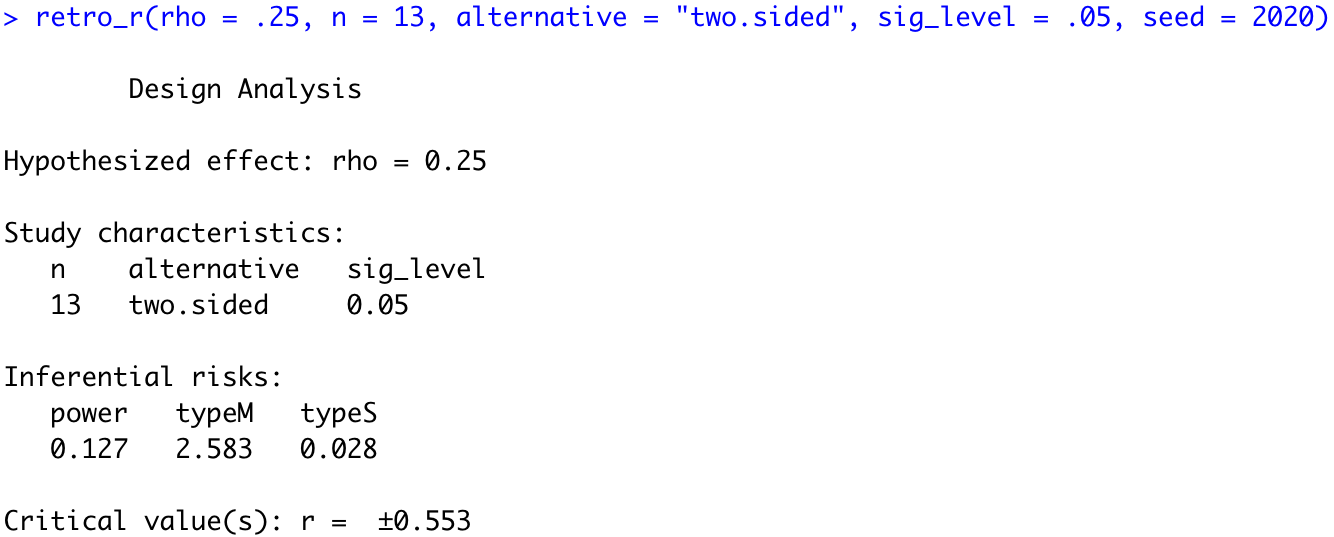
\includegraphics[height=5cm]{screens/retro}
\caption{Input and Output of the function \texttt{retro\_r()} for retrospective design analysis. Case study: \textcite{eisenbergerDoesRejectionHurt2003}. The plausible correlation coefficient is $\rho = .25$, the sample size is 13, and the statistical test is two-tailed. The option \texttt{seed} allows setting the random number generator to obtain reproducible results.}\label{fig:retro_r}
\end{figure}

In this research design, the critical values above which a statistically significant result is declared correspond to $r=\pm .55$ (Figure~\ref{fig:retro_r}).  These values are highlighted in Figure~\ref{fig:Plot_winner} as the vertical lines in the sampling distribution of correlation coefficients under the null hypothesis. Notice that the plausible effect size lies in the region of acceptance of the null hypothesis. Therefore, it is impossible to simultaneously find a statistically significant result and estimate an effect close to the plausible one ($\rho=.25$). The figure represents the so-called Winner’s curse: “the ‘lucky’ scientist who makes a discovery is cursed by finding an inflated estimate of that effect” \parencite{buttonPowerFailureWhy2013}.



\begin{knitrout}
\definecolor{shadecolor}{rgb}{0.98, 0.98, 1}\color{fgcolor}\begin{figure}[!h]

{\centering 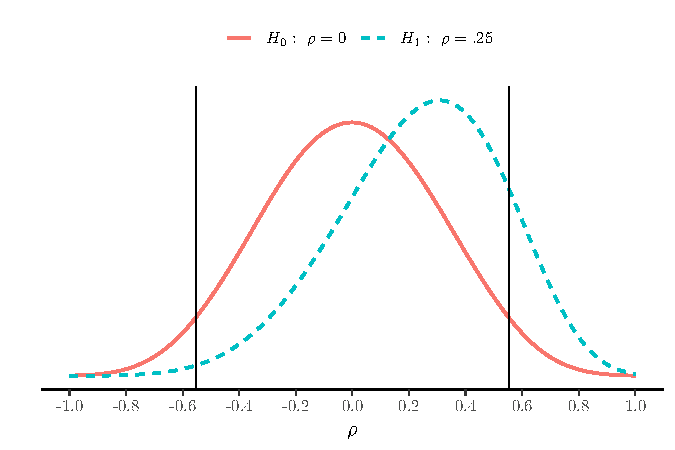
\includegraphics[width=\maxwidth]{figure/Plot_winner-1} 

}

\caption[Winner's course]{Winner's course. H$_0$ = Null Hypothesis, H$_1$ = Alternative Hypothesis. When sample size, directionality of the test and Type I error probability are set, also the smallest effect size above which is possible to find a statistically significant result is set. In this case, the plausible effect size, $\rho=.25$, lies in the region where it is not possible to reject H$_0$ (the region delimited by the two vertical lines). Thus, it is impossible to simultaneously find a statistically significant result and an effect close to the plausible one. In other words, a statistically significant effect must exaggerate the plausible effect size.}\label{fig:Plot_winner}
\end{figure}


\end{knitrout}

%----------------------------------------------------------------------------------%
%-------------------         Prospective Design Analysis         ------------------%
%----------------------------------------------------------------------------------%

\subsection{Prospective Design Analysis}

Ideally, Type M and Type S errors should be considered in the design phase of a study during the decision-making process regarding the experimental protocol. At this stage, prospective design analysis can be used as a sample size planning strategy which aims to minimize Type M and Type S errors in the upcoming study.

Imagine that we were part of the research team in the previous case study exploring the relationship between activity in the Anterior Cerebral Cortex and perceived distress. When drafting the research protocol, we face the inevitable discussion on how many participants we are going to recruit. This choice depends on available resources, type of study design, constraints of various nature and, importantly, the plausible magnitude and direction of the phenomenon that we are going to study. As previously mentioned, deciding on a plausible effect size is a fundamental step which requires great effort and should not be done by trying different values only to obtain a more desirable sample size. Instead, proposing a plausible effect size is where the expert knowledge of the researcher can be formalized and can greatly contribute to the informativeness of the study that is being planned. For the sake of these examples, we adopt the previous consideration and we suppose that common agreement is reached on a plausible correlation coefficient to be around $\rho=.25$. Finally, we would like to leave open the possibility to explore whether the relationship goes in the opposite direction to the one hypothesized, so we decide to perform a two-tailed test.

We can implement the prospective design analysis using the function \texttt{pro\_r()} which inputs and outputs are displayed in Figure~\ref{fig:pro_r}. About 125 participants are necessary to have 80\% probability to detect an effect of at least $\rho=\pm .25$ if it actually exists. With this sample size, the Type S error is minimized and approximates zero. In this study design, the Type M error is 1.11 indicating that statistically significant results are on average exaggerated by 11\%. It is possible to notice that the critical values are $r=\pm .18$, further highlighting that our plausible effect size is actually included among those values that lead to the acceptance of the alternative hypothesis.



\begin{figure}[!h]
\centering
  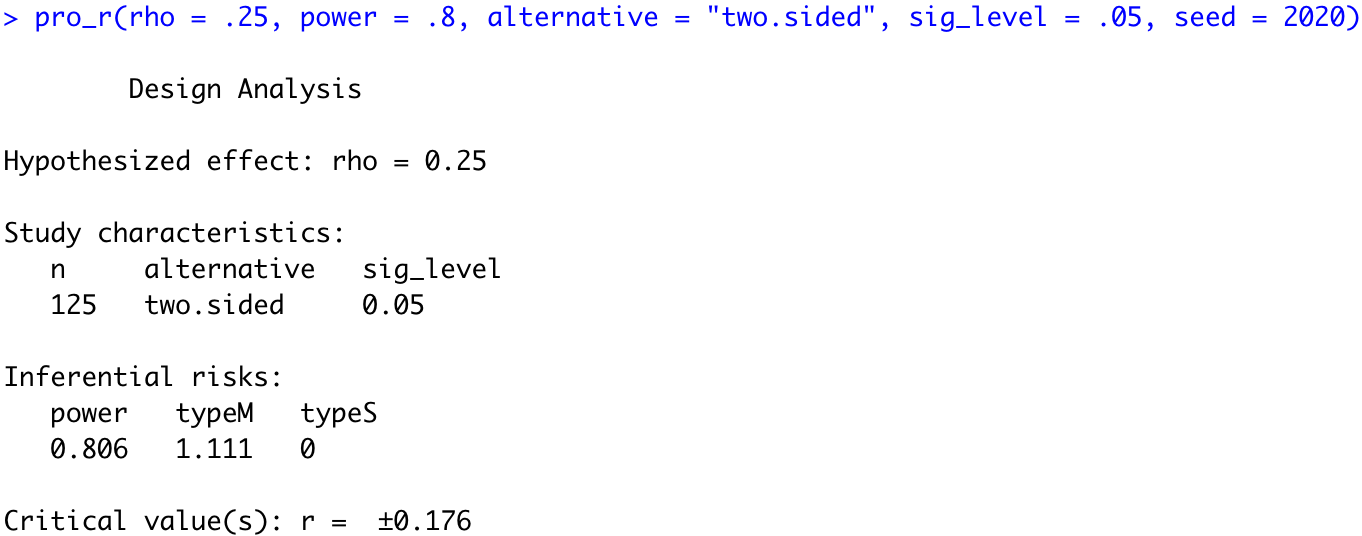
\includegraphics[height=5cm]{screens/pro}
\caption{Input and Output of the function \texttt{pro\_r()} for prospective design analysis. Plausible correlation coefficient is $\rho = .25$, statistical power is 80\% and the statistical test is two-tailed. The option \texttt{seed} allows setting the random number generator to obtain reproducible results.}\label{fig:pro_r}
\end{figure}

In a design analysis, it is advisable to investigate how the inferential risks would change according to different scenarios in terms of statistical power and plausible effect size. Changes in both these factors impact Type M and Type S errors. For example, maintaining the plausible correlation of $\rho = .25$, if we decrease statistical power from .80 to .60 only 76 participants are required (see Table~\ref{tab:Table_pro_r}). However, this is associated with an increased Type M error rate from 1.11 to 1.28. That is to say, with 76 subjects the plausible effect size will be on average overestimated by 28\%. Alternatively, imagine that we would like to maintain a statistical power of 80\%, what happens if the plausible effect size is slightly larger or smaller? The necessary sample size would spike to 344 for a $\rho=.15$  and decrease to 60 for $\rho=.35$. In both scenarios, the Type M error remains about 1.12, which reflects the more general point that for 80\% power, Type M error is around 1.10. In all these scenarios, Type S error is close to zero, hence not worrisome.





\begin{knitrout}
\definecolor{shadecolor}{rgb}{0.98, 0.98, 1}\color{fgcolor}\begin{table}[H]

\caption{\label{tab:Table_pro_r}Prospective design analysis in different scenarios of plausible effect size and statistical power.}
\centering
\begin{tabular}[t]{cccccc}
\toprule
\multicolumn{1}{c}{\textbf{$\bm{\rho}$}} & \multicolumn{1}{c}{\textbf{Power}} & \multicolumn{1}{c}{\textbf{Sample Size}} & \multicolumn{1}{c}{\textbf{Type M}} & \multicolumn{1}{c}{\textbf{Type S}} & \multicolumn{1}{c}{\textbf{Critical \textit{r} value}}\\
\midrule
0.25 & 0.6 & 76 & 1.280 & 0 & $\pm0.226$\\
0.15 & 0.8 & 344 & 1.116 & 0 & $\pm0.106$\\
0.35 & 0.8 & 60 & 1.115 & 0 & $\pm0.254$\\
\bottomrule
\multicolumn{6}{l}{\textit{Note: } In all cases, alternative  = \texttt{"two.sided"} and sig\_level = .05.}\\
\end{tabular}
\end{table}


\end{knitrout}

For completeness, Figure~\ref{fig:Plot_scenarios} summarizes the relationship between statistical power, Type M and Type S errors as a function of sample size in three scenarios of plausible correlation coefficients. We display the three values that \textcite{vulSuspiciouslyHighCorrelations2017} considered for correlations between fMRI measures and behavioural measures with different degrees of plausibility. An effect of $\rho=.75$ was deemed theoretically plausible but unrealistic, $\rho=.50$ was more plausible but optimistic, and $\rho=.25$ was more likely.  The curves illustrate a general point: Type M and Type S error increase with smaller sample sizes, smaller plausible effect sizes and lower statistical power. Also, the figure shows that statistical power, Type M and Type S errors are related to each other: as power increases, Type M and Type S errors decrease.

At first, it might seem that Type M and Type S errors are redundant with the information provided by statistical power. Even though they are related, we believe that Type M and Type S errors bring added value during the design phase of a research protocol because they facilitate a connection between how a study is planned and how results will actually be evaluated. That is to say, final results will comprise of a test statistics with an associated p-value and effect size measure. If the interest is maximizing the accuracy with which effects will be estimated, then Type M and Type S errors directly communicate the consequences of design choices on effect size estimation.



\begin{knitrout}
\definecolor{shadecolor}{rgb}{0.98, 0.98, 1}\color{fgcolor}\begin{figure}[!h]

{\centering 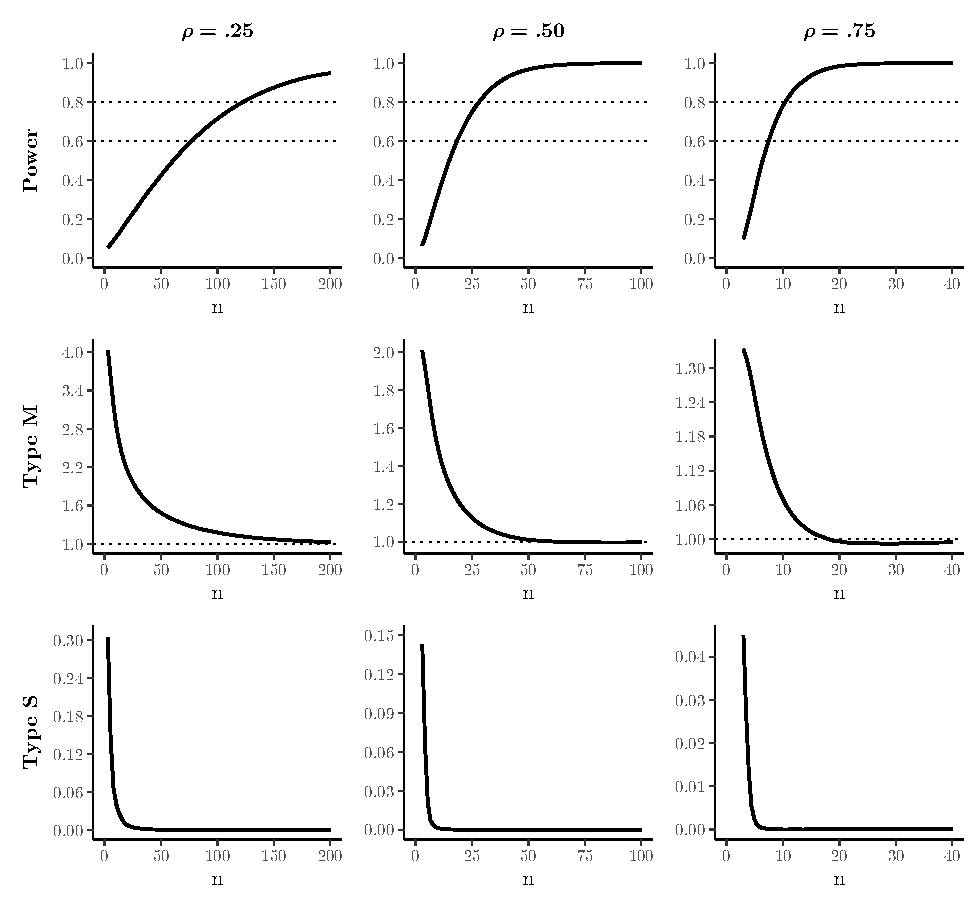
\includegraphics[width=\maxwidth]{figure/Plot_scenarios-1} 

}

\caption[How Type M, Type S and Statistical power vary as a function of sample size in three different scenarios of plausible effect size ($\rho=.25$, $\rho=.50$, $\rho=.75$)]{How Type M, Type S and Statistical power vary as a function of sample size in three different scenarios of plausible effect size ($\rho=.25$, $\rho=.50$, $\rho=.75$). Note that, for the sake of interpretability, we decided to use different scales for both the x-axis and y-axis in the three scenarios of plausible effect size.}\label{fig:Plot_scenarios}
\end{figure}


\end{knitrout}

%----------------------------------------------------------------------------------%
%------        Varying $\alpha$ levels and Hypotheses Directionality         ------%
%----------------------------------------------------------------------------------%

\section{Varying $\alpha$ levels and Hypotheses Directionality}

So far, we did not discuss two other important decisions that researchers have to take when designing a study: statistical significance threshold or $\alpha$ level, and directionality of the statistical test, one-tailed or two-tailed. In this section, we illustrate how different choices regarding these aspects impact Type M and Type S errors.

A lot has been written regarding the automatic adoption of a conventional $\alpha$ level of 5\% \parencite[e.g.,][]{gigerenzerNullRitualWhat2004, lakensJustifyYourAlpha2018}. This practice is increasingly discouraged, and researchers are invited to think about the best trade-off between $\alpha$ level and statistical power, considering the aim of the study and available resources. The $\alpha$ level impacts Type M and Type S errors as much as it impacts statistical power. Everything else equal, Type M error increases with decreasing $\alpha$ level (i.e., negative relationship), whereas Type S error decreases with decreasing $\alpha$ level (i.e., positive relationship). To further illustrate the relation between Type M error and $\alpha$ level, let us take as an example the previous case study with a sample of 13 participants, plausible effect size $\rho=.25$ and two-tailed test. Table~\ref{tab:Table_alpha} shows that by lowering the $\alpha$ level from 10\% to .10\%, the critical values move from $r=\pm .48$  to $r=\pm .80$. This suggests that, with these new higher thresholds, the exaggeration of effects will be even more pronounced because effects have to be even larger to pass such higher critical values. Instead, the relationship between Type S error and $\alpha$ level can be clarified thinking that by lowering the statistical significance threshold, we are being more conservative to falsely reject the null hypothesis in general which implies that we are also being more conservative to falsely reject the null hypothesis in the wrong direction.



\begin{knitrout}
\definecolor{shadecolor}{rgb}{0.98, 0.98, 1}\color{fgcolor}\begin{table}[H]

\caption{\label{tab:Table_alpha}How changes in $\alpha$ level impact Power, Type M error, Type S error and critical values.}
\centering
\begin{tabular}[t]{ccccc}
\toprule
\multicolumn{1}{c}{\textbf{$\bm{\alpha}$-level}} & \multicolumn{1}{c}{\textbf{Power}} & \multicolumn{1}{c}{\textbf{Type M}} & \multicolumn{1}{c}{\textbf{Type S}} & \multicolumn{1}{c}{\textbf{Critical \textit{r} value}}\\
\midrule
0.100 & 0.212 & 2.369 & 0.040 & $\pm0.476$\\
0.050 & 0.127 & 2.583 & 0.028 & $\pm0.553$\\
0.010 & 0.035 & 2.977 & 0.011 & $\pm0.684$\\
0.005 & 0.021 & 3.088 & 0.014 & $\pm0.726$\\
0.001 & 0.005 & 3.340 & 0.000 & $\pm0.801$\\
\bottomrule
\multicolumn{5}{l}{\textit{Note: } In all cases, $\rho=.25$, n = 13, and alternative  = \texttt{"two.sided"}.}\\
\end{tabular}
\end{table}


\end{knitrout}

Another important choice in study design is the directionality of the test (i.e., one-tailed or two-tailed).  Design analysis invites reasoning on the plausible effect size and hypothesizing the direction of the effect, not only its magnitude. So why should a researcher perform non-directional statistical tests when there is a hypothesized direction? Performing a two-tailed test leaves open the possibility to find an unexpected result in the opposite direction \parencite{cohenStatisticalPowerAnalysis1988}, a possibility which may be of special interest for preliminary exploratory studies. However, in more advanced stages of a research program (i.e., confirmatory study), directional hypotheses benefit from higher statistical power and lower Type M error rates (Figure~\ref{fig:Plot_hypothesis}). As an example, let us consider the differences between a two-tailed test and a one-tailed test in the previous case study. We can perform a new prospective design analysis (Figure~\ref{fig:pro_r2}) with a plausible correlation of $\rho=.25$, 80\% statistical power, but this time setting the argument \texttt{alternative} in the R function to \texttt{“greater”}. A comparison of the two prospective design analyses, Figure~\ref{fig:pro_r} and Figure~\ref{fig:pro_r2}, suggests that the same Type M error rate of about 10\% is guaranteed with 94 participants, instead of the 125 subjects necessary with a two-tailed test. Note that Type S error is not possible in directional statistical tests. Indeed, all the statistically significant results are obtainable only in the hypothesized direction, not the opposite one.



\begin{knitrout}
\definecolor{shadecolor}{rgb}{0.98, 0.98, 1}\color{fgcolor}\begin{figure}[!h]

{\centering 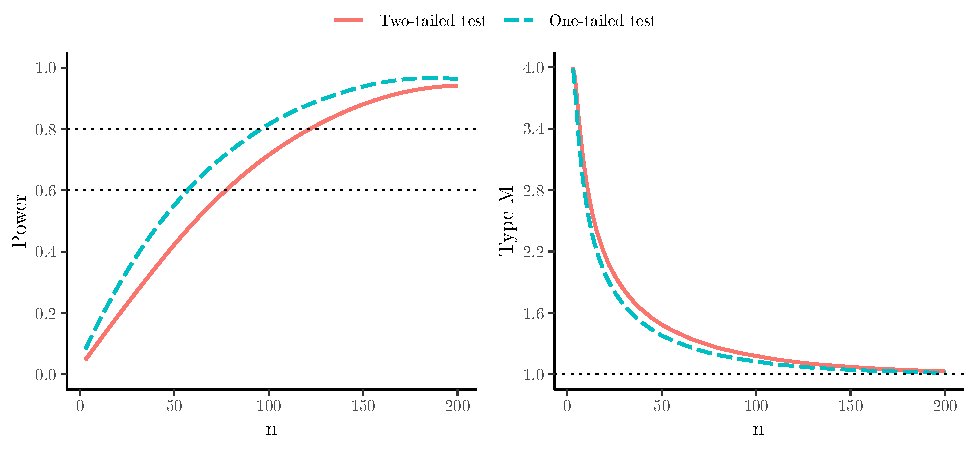
\includegraphics[width=\maxwidth]{figure/Plot_hypothesis-1} 

}

\caption[Comparison of Type M error rate and Power level between one-tailed and two-tailed test with $\rho = .25$, $\alpha = .05$]{Comparison of Type M error rate and Power level between one-tailed and two-tailed test with $\rho = .25$, $\alpha = .05$. n = sample size. }\label{fig:Plot_hypothesis}
\end{figure}


\end{knitrout}




\begin{figure}[!h]
\centering
  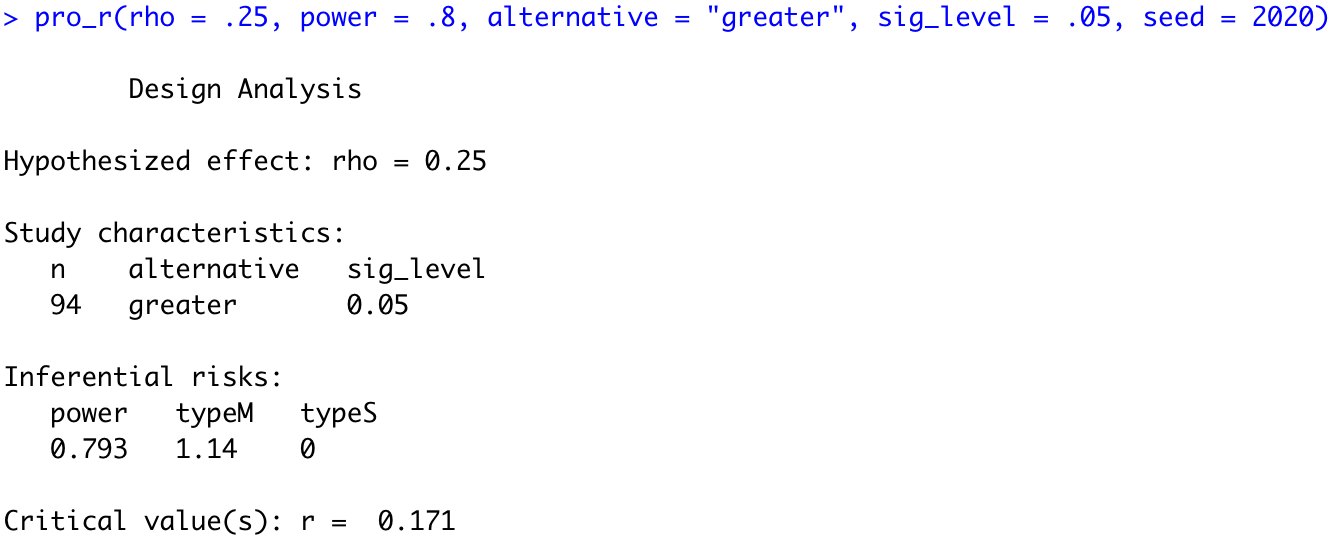
\includegraphics[height=5cm]{screens/pro2}
\caption{Input and Output of the function \texttt{pro\_r()} for prospective design analysis. Plausible correlation coefficient is $\rho = .25$, statistical power is 80\% and the statistical test is one-tailed.}\label{fig:pro_r2}
\end{figure}

Valid conclusions require decisions on test directionality and $\alpha$ level to be taken a priori, not while data are being analyzed \parencite{cohenStatisticalPowerAnalysis1988}. These decisions can take place during a prospective design analysis, which aligns with the increasing interest in psychological science to transparently communicate and justify design choices through studies’ preregistration in public repositories (e.g., Open Science Framework; Aspredicted.com). Preregistration of studies’ protocol is particularly valuable for researchers endorsing an error statistics philosophy of science, where the evaluation of research results takes into account the severity with which claims are tested \parencite{lakensValuePreregistrationPsychological2019,mayoStatisticalInferenceSevere2018}. Severity depends on the degree to which a research protocol tries to falsify a claim. For example, a one-tailed statistical test provides greater severity than a two-tailed statistical test. As noted by \textcite{lakensValuePreregistrationPsychological2019}, preregistration is important to openly share a priori decisions, such as test-directionality, providing valuable information for researchers interested in evaluating the severity of research claims.

%----------------------------------------------------------------------------------%
%-----------------    Publication Bias and Significance Filter    -----------------%
%----------------------------------------------------------------------------------%


\section{Publication Bias and Significance Filter}

On a concluding note, we would like to clarify the relationship of Design Analysis with publication bias and the statistical significance filter.

While publication bias and Type M and Type S errors are related, they operate at two different levels. Publication bias refers to a publication system that favours statistically significant results over non-statistically significant findings. This phenomenon alone cannot explain the presence of exaggerated effects. Imagine if all studies in the literature were conducted with high statistical power, then statistically significant findings would probably not be so extreme. The problem of exaggerated effect sizes in the literature can be explained only by a combination of publication bias with studies that have low statistical power. As previously shown, statistical power and Type M and Type S errors are related to each other: low statistical power corresponds to higher Type M and Type S errors.

The critical element is the application of the statistical significance filter without taking into account statistical power. Design Analysis per se does not solve this issue but, instead, it allows us to recognize its problematic consequences. In the same way as statistical power is a characteristic of a study design, so are Type M and Type S errors, however, the two are qualitatively different in terms of the kind of reasoning they favour. Statistical power is defined in terms of probability of rejecting the Null hypothesis and, even though this is based on an effect size of interest, the relationship “low power - high possibility of exaggeration” may not be straightforward for everyone. Instead, Type M and Type S errors directly quantify the possible exaggeration. Furthermore, their consideration protects against another possible pitfall. When in a study a statistically significant result is found and the associated effect size estimate is large, the finding could be interpreted as robust and impressive. However, this interpretation is not always appropriate. Here, the missing piece of information is  statistical power. If power is considered, researchers would realize that a large effect was found in a context where there was a low probability to find it. But this interpretation is not explicitly stating an important aspect: in these conditions, the only way to find a statistically significant result is by overestimating the true effect. On the contrary, this consequence becomes immediately clear once Type M and Type S errors are considered retrospectively. Similarly, considering Type M and Type S prospectively favours reasoning in terms of effect size rather than the probability of rejecting the null hypothesis when setting the sample size in a design analysis.


%----------------------------------------------------------------------------------%
%--------------------         Discussion and Conclusion         -------------------%
%----------------------------------------------------------------------------------%

\section{Discussion and Conclusion}

In the scientific community, it is quite widespread the idea that the literature is affected by a problem with effect size exaggeration. This issue is usually explained in terms of studies’ low statistical power combined with the use of thresholds of statistical significance \parencite{buttonPowerFailureWhy2013,ioannidisWhyMostDiscovered2008,ioannidisEmergenceLargeTreatment2013,laneEstimatingEffectSize1978,yarkoniBigCorrelationsLittle2009,youngWhyCurrentPublication2008}. Statistically significant results can be obtained even in underpowered studies and it is precisely in these cases that we should worry the most about issues of overestimation. Type M and Type S errors quantify and highlight the inferential risks directly in terms of effect size estimation, which are implied by the concept of statistical power but might not be recognizable outright. So far, only a handful of papers explicitly mentioned Type M and Type S errors \parencite{altoeEnhancingStatisticalInference2020,gelmanFailureNullHypothesis2018,gelmanTypeErrorMight2017,gelmanRetrospectiveDesignAnalysis2013,gelmanPowerCalculationsAssessing2014,gelmanTypeErrorRates2000,luNoteTypeErrors2018,vasishthStatisticalSignificanceFilter2018}. With the broader goal of facilitating their consideration in psychological science, in the present contribution we illustrated how Type M and Type S errors are considered in a design analysis using one of the most common effect size measures in psychology, Pearson correlation coefficient.

Peculiar to design analysis is the focus on the implications of design choices on effect sizes estimation rather than statistical significance only. We illustrated how Type M and Type S errors can be taken into account with a \emph{prospective design analysis}. In the planning stage of a research project, design analysis has the potential to increase researchers’ awareness of the consequences that their sample size choices have on uncertainty about final estimates of the effects. This favours reasoning in similar terms to those in which results will be evaluated, that is to say, effect size estimation. But understanding the inferential risks in a study design is also beneficial once results are obtained. We presented \emph{retrospective design analysis} on a published study, and the same process can be useful for studies in general, especially those ending without the necessary sample size to maximize statistical power and minimize Type M and Type S errors. In all cases, presenting their values effectively communicates the uncertainty of the results. In particular, Type M and Type S errors put a red flag when results are statistically significant, but the effect size could be largely overestimated and in the wrong direction. Finally, both prospective and retrospective design analysis favours cumulative science encouraging the incorporation of expert knowledge in the definition of the plausible effect sizes.

It is important to remark that even if Design Analysis is based on the definition of a plausible effect size, a best practice should be to conduct multiple Design Analyses by considering different scenarios which  include different plausible effect sizes and levels of power to maximize the informativeness of both a prospective and a retrospective analysis.

To make design analysis accessible to the research community, we provide the R functions to perform prospective design analysis and retrospective design analysis for Pearson correlation coefficient \url{https://osf.io/9q5fr/} together with a short guide on how to use the R functions and a summary of the examples presented in this contribution (Appendix~\ref{sec:appendix_b}).

Finally, prospective design analysis could contribute to better research design, however many other important factors were not considered in this contribution. For example, the validity and reliability of measurements should be at the forefront in research design, and careful planning of the entire research protocol is of utmost importance. Future works could tackle some of these shortcomings for example, including an analysis of the quality of measurement on the estimates of Type M and Type S errors. Also, we believe that it would be valuable to provide extension of design analysis for other common effect size measures with the development of statistical software packages that could be directly used by researchers. Moreover, design analysis on Pearson correlation can be easily extended to the multivariate case where multiple predictors are considered. Lastly, design analysis is not limited to the Neyman-Pearson framework but can be considered also within other statistical approaches such as Bayesian approach. Future works could implement design analysis to evaluate the inferential risks related to the use of Bayes Factors and Bayesian Credibility Intervals.

Summarizing, choices regarding studies’ design impact effect size estimation and Type M (magnitude) error and Type S (sign) error allow to directly quantify these inferential risks. Their consideration in a prospective design analysis increases awareness of what are the consequences of sample size choice reasoning in similar terms to those used in results evaluation. Instead, retrospective design analysis provides further guidance on interpreting research results. More broadly, design analysis reminds researchers that statistical inference should start before data collection and does not end when results are obtained.

\phantomsection
\addcontentsline{toc}{section}{Bibliography}
\printbibliography
%\bibliography{Paper_main}

\clearpage

\appendix
\titleformat{\section}{\normalfont\Large\bfseries}{\setappendix}{0em}{}
\renewcommand\thefigure{\thesection.\arabic{figure}}
\renewcommand\theequation{\thesection.\arabic{equation}}
%----------------------------------------------------------------------------------%
%---------------------------       Appendix A      --------------------------------%
%----------------------------------------------------------------------------------%
\begin{refsection}

\section{Pearson Correlation and Design Analysis}\label{sec:appendix_a}
\setcounter{figure}{0}
\setcounter{equation}{0}
\setcounter{footnote}{0}

To conduct a design analysis, it is necessary to know the sampling distribution of the effect of interest. That is, the distribution of effects we would observe if \emph{n} observations were sampled over and over again from a population with a given effect. This allows us, in turns, to evaluate the sampling distribution of the test statistic of interest not only under the Null-Hypothesis ($H_0$), but also under the alternative Hypothesis ($H_1$), and  thus to compute the statistical power and inferential risks of the study considered.

Regarding Pearson's correlation between two normally distributed variables, the sampling distribution is bounded between -1 and 1 and its shape depends on the values of $\rho$ and \emph{n}, respectively the population correlation value and the sample size. The sampling distribution is approximately Normal if $\rho = 0$. Whereas, for positive or negative values of $\rho$, it is negatively skewed or positively skewed, respectively. Skewness is greater for higher absolute values of $\rho$ but decreases when larger sample sizes are considered. In Figure~\ref{fig:Plot_sampling_rho}, correlation sampling distributions are presented for increasing values of $\rho$ and fixed sample size ($n = 30$).





\begin{knitrout}
\definecolor{shadecolor}{rgb}{0.98, 0.98, 1}\color{fgcolor}\begin{figure}[!h]

{\centering 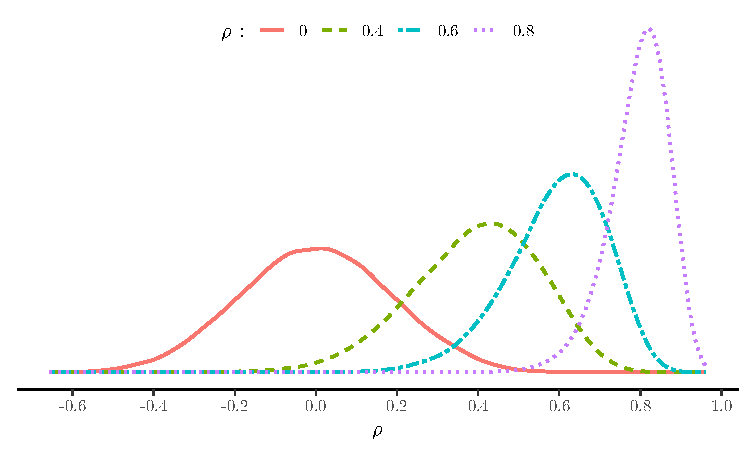
\includegraphics[width=\maxwidth]{figure/Plot_sampling_rho-1} 

}

\caption[Pearson Correlation coefficient sampling distributions for increasing values of $\rho$ and fixed sample size ($n = 30$)]{Pearson Correlation coefficient sampling distributions for increasing values of $\rho$ and fixed sample size ($n = 30$)}\label{fig:Plot_sampling_rho}
\end{figure}


\end{knitrout}

In the following paragraphs, we consider the consequence of Pearson's correlation sampling distribution on statistical inference and the behaviour of Type M and Type S errors as a function of statistical power.

\subsection{Statistical inference}

To test a hypothesis or to derive confidence intervals, the sampling distribution of the test statistic of interest must follow a known distribution. In the case of $H_0:\ \rho = 0$, the sample correlation is approximately normally distributed with Standard Error: $\text{SE}(r) = \sqrt{(1-r^2)/(n-2)}$. Thus, statistical inference is performed considering the test statistic:
\begin{equation}
  t = \frac{r}{\text{SE}(r)} = r \sqrt{\frac{n-2}{1-r^2}},
\end{equation}
that follows a \emph{t}-distribution with $df = n-2$.

However, in the case of $\rho \neq 0$, the sample correlation is no longer normally distributed. As we have previously seen, the sampling distribution is skewed for large values of $\rho$ and small sample sizes. Thus, the test statistic of interest does not follow a \emph{t}-distribution.\footnote{Note that the \emph{t}-distribution is defined as the distribution of a random variable T where $T = \frac{Z}{\sqrt{V/df}}$. With \emph{Z} a standard Normal, \emph{V} a Chi-squared distribution with \emph{df} the degrees of freedom. Thus, if the sample correlation is no longer approximately normally distributed the test-statistic is no longer \emph{t}-distributed.} To overcome this issue, the Fisher transformation was introduced \parencite{fisherFrequencyDistributionValues1915}:
\begin{equation}
  F(r) = \frac{1}{2}\ ln \frac{1+r}{1-r} = \text{arctanh}(r).
\end{equation}
Applying this transformation, the resulting sampling distribution is approximately Normal with $\text{mean} = F(\rho)$ and $\text{SE} = \frac{1}{\sqrt{n-3}}$. Thus, the test statistic follows a standard Normal distribution and statistical inference is performed considering the \emph{Z}-scores.

Alternatively, other methods can be used to obtain reliable results, for example, Monte Carlo simulation. Monte Carlo simulation is based on random sampling to approximate the quantities of interest. In the case of correlation, \emph{n} observations are iteratively simulated from a bivariate Normal distribution with a given $\rho$, and the observed correlation is considered. As the number of iterations increases, the distribution of simulated correlation values approximates the actual correlation sampling distribution and it can be used to compute the quantities of interest.

Although Monte Carlo methods are more computationally demanding than analytic solutions, this approach allows us to obtain reliable results in a wider range of conditions even when no closed-form solutions are available. For these reasons, the functions \texttt{pro\_r()} and \texttt{retro\_r()}, presented in this paper, are based on Monte Carlo simulation to compute power, Type M, and Type S error values. This guarantees a more general framework where other future applications can be easily integrated into the functions.

\subsection{Type M and Type S errors}

Design Analysis was first introduced by \textcite{gelmanPowerCalculationsAssessing2014} assuming that the sampling distribution of the test statistic of interest follows a \emph{t}-distribution. This is the case, for example, of Cohen's \emph{d} effect size. Cohen's \emph{d} is used to measure the mean difference between two groups on a continuous outcome. The behaviour of Type M and Type S errors as a function of statistical power in the case of Cohen's \emph{d} is presented in Figure~\ref{fig:Plot_cohen}.



\begin{knitrout}
\definecolor{shadecolor}{rgb}{0.98, 0.98, 1}\color{fgcolor}\begin{figure}[!h]

{\centering 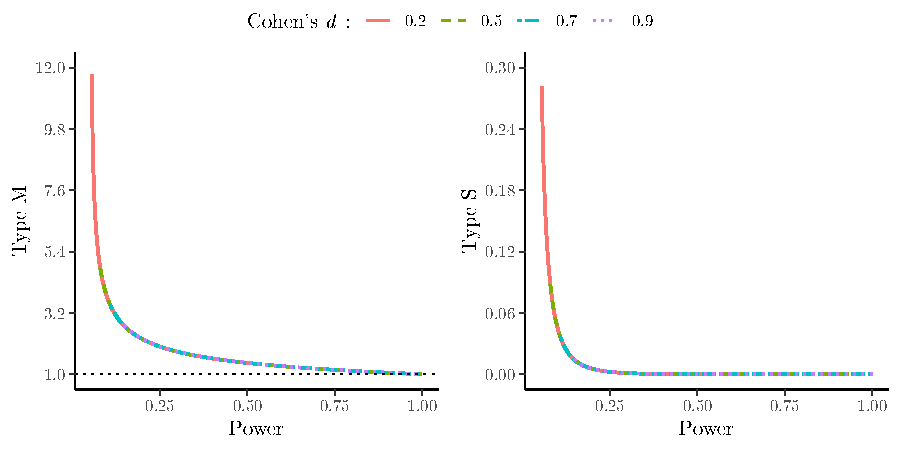
\includegraphics[width=\maxwidth]{figure/Plot_cohen-1} 

}

\caption[The behaviour of Type M and Type S errors as a function of statistical power in the case of Cohen's \emph{d}]{The behaviour of Type M and Type S errors as a function of statistical power in the case of Cohen's \emph{d}. Note that the four lines are overlapping.}\label{fig:Plot_cohen}
\end{figure}


\end{knitrout}


For different values of hypothetical population effect size (\emph{d} = .2, .5, .7, .9), we can observe that, for high levels of power, Type S and Type M errors are low. Conversely, the Type S and Type M errors are high for low values of power. As expected, the relation between power and inferential errors is not influenced by the value of \emph{d} (i.e., the four lines are overlapping). Limit cases are obtained for power = 1 and 0.05 (note that the lowest value of power is given by the alpha value chosen as the statistical significance threshold). In the former case, Type S error is 0 and Type M error is 1. In the latter case, Type S error is 0.5 and the Type M error value goes to infinity.

In the case of Pearson's Correlation, we noted above that the sampling distribution is skewed for large values of $\rho$ and small sample sizes. Moreover, the support is bounded between -1 and 1. Thus, the relations between power, Type M, and Type S error are influenced by the value of the hypothetical population effect size (see Figure~\ref{fig:Plot_rho}).



\begin{knitrout}
\definecolor{shadecolor}{rgb}{0.98, 0.98, 1}\color{fgcolor}\begin{figure}[!h]

{\centering 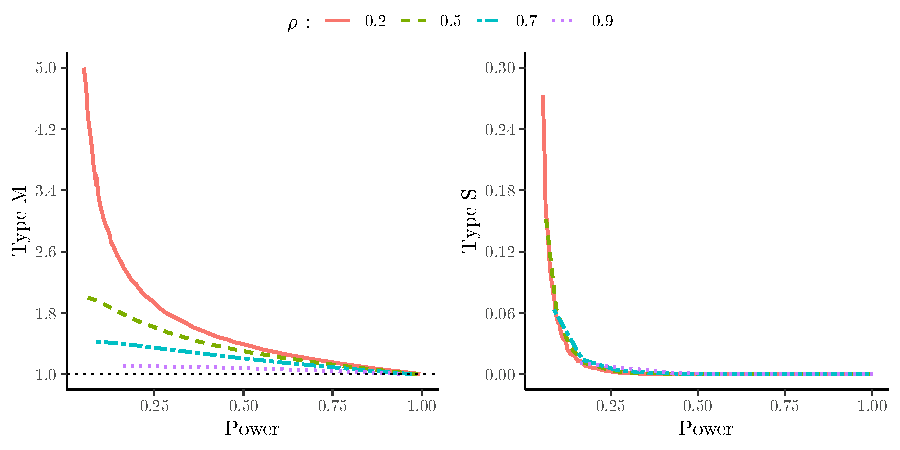
\includegraphics[width=\maxwidth]{figure/Plot_rho-1} 

}

\caption[The behaviour of Type M and Type S errors as a function of statistical power in the case of Pearson's correlation $\rho$]{The behaviour of Type M and Type S errors as a function of statistical power in the case of Pearson's correlation $\rho$.}\label{fig:Plot_rho}
\end{figure}


\end{knitrout}


We can observe how, for different values of correlation ($\rho$ = .2, .5, .7, .9), Type M error increases at different rates when the power decrease, whereas Type S error follows a consistent pattern (note that differences are due to numerical approximation). We can intuitively explain this behaviour considering that, for low levels of power, the sampling distribution includes a wider range of correlation values. However, correlation values can not exceed the value 1 and therefore the distribution becomes progressively more skewed. This does not influence the proportion of statistically significant sampled correlations with the incorrect sign (Type S error), but it affects the mean absolute value of statistically significant sampled correlations (used to compute Type M error). In particular, the sampling distribution for greater values of $\rho$ becomes skewed more rapidly and thus Type-M error increases at a lower rate.

Finally, since the correlation values are bounded, Type-M error for a given value of $\rho$ can hypothetically increase only to a maximum value given by $\frac{1}{\rho}$. For example, for $\rho = .5$ the maximum Type-M error is 2 as $.5\times 2 = 1$ (i.e., the maximum correlation value).

In this appendix, we discussed for completeness the implications of conducting a Design Analysis in the case of Pearson's correlation effect size. We considered extreme scenarios that are unlikely to happen in real research settings. Nevertheless, we thought this was important for evaluating the statistical behaviour and properties of Type M and Type S error in the case of Pearson's correlation as well as helping researchers to deeply understand Design Analysis.

\clearpage

%----------------------------------------------------------------------------------%
%---------------------------       Appendix B      --------------------------------%
%----------------------------------------------------------------------------------%

\section{R Functions for Design Analysis\\ with Pearson Correlation}\label{sec:appendix_b}
\setcounter{figure}{0}
\setcounter{equation}{0}

Here we describe the R functions defined to perform a prospective and retrospective design analysis in the case of Pearson correlation. First, we give instructions on how to load and use the functions. Subsequently, we provide the code to reproduce examples included in the article.

These functions can be used as a base to further develop design analysis in more complex scenarios that were beyond the aim of the paper.

\subsection{R functions}

The code of the functions is available in the file \texttt{Design\_analysis\_r.R} at \url{https://osf.io/9q5fr/}.

After downloading the file \texttt{Design\_analysis\_r.R}, run the line indicating the correct path where the file was saved:
\begin{knitrout}
\definecolor{shadecolor}{rgb}{0.98, 0.98, 1}\color{fgcolor}\begin{kframe}
\begin{alltt}
\hlkwd{source}\hlstd{(}\hlstr{"<your_path>/Design_analyisis_r.R"}\hlstd{)}
\end{alltt}
\end{kframe}
\end{knitrout}
The script will automatically load in your workspace the functions and two required R-package: \texttt{MASS} \parencite{venablesModernAppliedStatistics2002} and \texttt{docstring} \textcite{kurkiewiczDocstringProvidesDocstring2017}. If you don't have them already installed, run the line \texttt{install.packages(c("MASS","docstring"))}.

The R functions are:
\begin{itemize}
\item{\texttt{retro\_r()} for retrospective design analysis. Given the hypothetical population correlation value and sample size, this function performs a retrospective design analysis according to the defined alternative hypothesis and significance level. Power level, Type-M error, and Type-S error are computed together with the critical correlation value (i.e., the minimum absolute correlation value that would result significant).}
\begin{knitrout}
\definecolor{shadecolor}{rgb}{0.98, 0.98, 1}\color{fgcolor}\begin{kframe}
\begin{alltt}
\hlkwd{retro_r}\hlstd{(rho, n,} \hlkwc{alternative} \hlstd{=} \hlkwd{c}\hlstd{(}\hlstr{"two.sided"}\hlstd{,} \hlstr{"less"}\hlstd{,} \hlstr{"greater"}\hlstd{),}
    \hlkwc{sig_level} \hlstd{=} \hlnum{0.05}\hlstd{,} \hlkwc{B} \hlstd{=} \hlnum{10000}\hlstd{,} \hlkwc{seed} \hlstd{=} \hlkwa{NULL}\hlstd{)}
\end{alltt}
\end{kframe}
\end{knitrout}

\item{\texttt{pro\_r()} for prospective design analysis. Given the hypothetical population correlation value and the required power level, this function performs a prospective design analysis according to the defined alternative hypothesis and significance level. The required sample size is computed together with the associated Type-M error, Type-S error, and the critical correlation value.
\begin{knitrout}
\definecolor{shadecolor}{rgb}{0.98, 0.98, 1}\color{fgcolor}\begin{kframe}
\begin{alltt}
\hlkwd{pro_r}\hlstd{(rho,} \hlkwc{power} \hlstd{=} \hlnum{0.8}\hlstd{,} \hlkwc{alternative} \hlstd{=} \hlkwd{c}\hlstd{(}\hlstr{"two.sided"}\hlstd{,} \hlstr{"less"}\hlstd{,} \hlstr{"greater"}\hlstd{),}
    \hlkwc{sig_level} \hlstd{=} \hlnum{0.05}\hlstd{,} \hlkwc{range_n} \hlstd{=} \hlkwd{c}\hlstd{(}\hlnum{1}\hlstd{,} \hlnum{1000}\hlstd{),} \hlkwc{B} \hlstd{=} \hlnum{10000}\hlstd{,} \hlkwc{tol} \hlstd{=} \hlnum{0.01}\hlstd{,}
    \hlkwc{display_message} \hlstd{=} \hlnum{FALSE}\hlstd{,} \hlkwc{seed} \hlstd{=} \hlkwa{NULL}\hlstd{)}
\end{alltt}
\end{kframe}
\end{knitrout}
}
\end{itemize}

For further details about function arguments, run the line \texttt{docstring(retro\_r)} or \texttt{docstring(pro\_r)}. This creates a documentation similar to the help page of R functions.

\textbf{Note:} two other functions are defined in the script and will be loaded in your workspace (i.e., \texttt{compute\_crit\_r()} and \texttt{print.design\_analysus}). This are internal functions that should not be used directly by the user.

\subsection{Examples code}

Below we report the code to reproduce the examples included in the article.

\begin{knitrout}
\definecolor{shadecolor}{rgb}{0.98, 0.98, 1}\color{fgcolor}\begin{kframe}
\begin{alltt}
\hlcom{# Example from Figure 1}

\hlkwd{retro_r}\hlstd{(}\hlkwc{rho} \hlstd{=} \hlnum{0.25}\hlstd{,} \hlkwc{n} \hlstd{=} \hlnum{13}\hlstd{,} \hlkwc{alternative} \hlstd{=} \hlstr{"two.sided"}\hlstd{,} \hlkwc{sig_level} \hlstd{=} \hlnum{0.05}\hlstd{,} \hlkwc{seed} \hlstd{=} \hlnum{2020}\hlstd{)}
\end{alltt}
\end{kframe}
\end{knitrout}

\begin{knitrout}
\definecolor{shadecolor}{rgb}{0.98, 0.98, 1}\color{fgcolor}\begin{kframe}
\begin{alltt}
\hlcom{# Example from Figure 3}

\hlkwd{pro_r}\hlstd{(}\hlkwc{rho} \hlstd{=} \hlnum{0.25}\hlstd{,} \hlkwc{power} \hlstd{=} \hlnum{0.8}\hlstd{,} \hlkwc{alternative} \hlstd{=} \hlstr{"two.sided"}\hlstd{,} \hlkwc{sig_level} \hlstd{=} \hlnum{0.05}\hlstd{,} \hlkwc{seed} \hlstd{=} \hlnum{2020}\hlstd{)}
\end{alltt}
\end{kframe}
\end{knitrout}

\begin{knitrout}
\definecolor{shadecolor}{rgb}{0.98, 0.98, 1}\color{fgcolor}\begin{kframe}
\begin{alltt}
\hlcom{# Example from Figure 6}

\hlkwd{pro_r}\hlstd{(}\hlkwc{rho} \hlstd{=} \hlnum{0.25}\hlstd{,} \hlkwc{power} \hlstd{=} \hlnum{0.8}\hlstd{,} \hlkwc{alternative} \hlstd{=} \hlstr{"two.sided"}\hlstd{,} \hlkwc{sig_level} \hlstd{=} \hlnum{0.05}\hlstd{,} \hlkwc{seed} \hlstd{=} \hlnum{2020}\hlstd{)}
\end{alltt}
\end{kframe}
\end{knitrout}

\begin{knitrout}
\definecolor{shadecolor}{rgb}{0.98, 0.98, 1}\color{fgcolor}\begin{kframe}
\begin{alltt}
\hlcom{# Examples from Table 1}

\hlkwd{pro_r}\hlstd{(}\hlkwc{rho} \hlstd{=} \hlnum{0.25}\hlstd{,} \hlkwc{power} \hlstd{=} \hlnum{0.6}\hlstd{,} \hlkwc{alternative} \hlstd{=} \hlstr{"two.sided"}\hlstd{,} \hlkwc{sig_level} \hlstd{=} \hlnum{0.05}\hlstd{,} \hlkwc{seed} \hlstd{=} \hlnum{2020}\hlstd{)}

\hlkwd{pro_r}\hlstd{(}\hlkwc{rho} \hlstd{=} \hlnum{0.15}\hlstd{,} \hlkwc{power} \hlstd{=} \hlnum{0.8}\hlstd{,} \hlkwc{alternative} \hlstd{=} \hlstr{"two.sided"}\hlstd{,} \hlkwc{sig_level} \hlstd{=} \hlnum{0.05}\hlstd{,} \hlkwc{seed} \hlstd{=} \hlnum{2020}\hlstd{)}

\hlkwd{pro_r}\hlstd{(}\hlkwc{rho} \hlstd{=} \hlnum{0.35}\hlstd{,} \hlkwc{power} \hlstd{=} \hlnum{0.8}\hlstd{,} \hlkwc{alternative} \hlstd{=} \hlstr{"two.sided"}\hlstd{,} \hlkwc{sig_level} \hlstd{=} \hlnum{0.05}\hlstd{,} \hlkwc{seed} \hlstd{=} \hlnum{2020}\hlstd{)}
\end{alltt}
\end{kframe}
\end{knitrout}

\begin{knitrout}
\definecolor{shadecolor}{rgb}{0.98, 0.98, 1}\color{fgcolor}\begin{kframe}
\begin{alltt}
\hlcom{# Examples from Table 2}

\hlkwd{retro_r}\hlstd{(}\hlkwc{rho} \hlstd{=} \hlnum{0.25}\hlstd{,} \hlkwc{n} \hlstd{=} \hlnum{13}\hlstd{,} \hlkwc{alternative} \hlstd{=} \hlstr{"two.sided"}\hlstd{,} \hlkwc{sig_level} \hlstd{=} \hlnum{0.1}\hlstd{,} \hlkwc{seed} \hlstd{=} \hlnum{2020}\hlstd{)}

\hlkwd{retro_r}\hlstd{(}\hlkwc{rho} \hlstd{=} \hlnum{0.25}\hlstd{,} \hlkwc{n} \hlstd{=} \hlnum{13}\hlstd{,} \hlkwc{alternative} \hlstd{=} \hlstr{"two.sided"}\hlstd{,} \hlkwc{sig_level} \hlstd{=} \hlnum{0.05}\hlstd{,} \hlkwc{seed} \hlstd{=} \hlnum{2020}\hlstd{)}

\hlkwd{retro_r}\hlstd{(}\hlkwc{rho} \hlstd{=} \hlnum{0.25}\hlstd{,} \hlkwc{n} \hlstd{=} \hlnum{13}\hlstd{,} \hlkwc{alternative} \hlstd{=} \hlstr{"two.sided"}\hlstd{,} \hlkwc{sig_level} \hlstd{=} \hlnum{0.01}\hlstd{,} \hlkwc{seed} \hlstd{=} \hlnum{2020}\hlstd{)}

\hlkwd{retro_r}\hlstd{(}\hlkwc{rho} \hlstd{=} \hlnum{0.25}\hlstd{,} \hlkwc{n} \hlstd{=} \hlnum{13}\hlstd{,} \hlkwc{alternative} \hlstd{=} \hlstr{"two.sided"}\hlstd{,} \hlkwc{sig_level} \hlstd{=} \hlnum{0.005}\hlstd{,} \hlkwc{seed} \hlstd{=} \hlnum{2020}\hlstd{)}

\hlkwd{retro_r}\hlstd{(}\hlkwc{rho} \hlstd{=} \hlnum{0.25}\hlstd{,} \hlkwc{n} \hlstd{=} \hlnum{13}\hlstd{,} \hlkwc{alternative} \hlstd{=} \hlstr{"two.sided"}\hlstd{,} \hlkwc{sig_level} \hlstd{=} \hlnum{0.001}\hlstd{,} \hlkwc{seed} \hlstd{=} \hlnum{2020}\hlstd{)}
\end{alltt}
\end{kframe}
\end{knitrout}

\printbibliography[heading=subbibliography, title = Appendix References ]
\end{refsection}

\clearpage
%----------------------------------------------------------------------------------%
%--------------------------    Session Information   ------------------------------%
%----------------------------------------------------------------------------------%


\section*{Session Information}

\begin{knitrout}
\definecolor{shadecolor}{rgb}{0.98, 0.98, 1}\color{fgcolor}\begin{kframe}
\begin{alltt}
\hlkwd{sessionInfo}\hlstd{(}\hlkwc{package} \hlstd{=} \hlkwa{NULL}\hlstd{)}
\end{alltt}
\begin{verbatim}
## R version 4.1.0 (2021-05-18)
## Platform: x86_64-pc-linux-gnu (64-bit)
## Running under: Ubuntu 18.04.5 LTS
## 
## Matrix products: default
## BLAS:   /usr/lib/x86_64-linux-gnu/blas/libblas.so.3.7.1
## LAPACK: /usr/lib/x86_64-linux-gnu/lapack/liblapack.so.3.7.1
## 
## locale:
##  [1] LC_CTYPE=en_US.UTF-8       LC_NUMERIC=C               LC_TIME=en_US.UTF-8       
##  [4] LC_COLLATE=en_US.UTF-8     LC_MONETARY=en_US.UTF-8    LC_MESSAGES=en_US.UTF-8   
##  [7] LC_PAPER=en_US.UTF-8       LC_NAME=C                  LC_ADDRESS=C              
## [10] LC_TELEPHONE=C             LC_MEASUREMENT=en_US.UTF-8 LC_IDENTIFICATION=C       
## 
## attached base packages:
## [1] grid      stats     graphics  grDevices utils     datasets  methods   base     
## 
## other attached packages:
##  [1] docstring_1.0.0  MASS_7.3-51.6    gtable_0.3.0     gridExtra_2.3    kableExtra_1.1.0
##  [6] forcats_0.5.0    stringr_1.4.0    dplyr_0.8.5      purrr_0.3.4      readr_1.3.1     
## [11] tidyr_1.0.2      tibble_3.0.1     ggplot2_3.3.0    tidyverse_1.3.0  knitr_1.28      
## 
## loaded via a namespace (and not attached):
##  [1] Rcpp_1.0.3          lubridate_1.7.8     lattice_0.20-38     assertthat_0.2.1   
##  [5] digest_0.6.25       R6_2.4.1            cellranger_1.1.0    backports_1.1.5    
##  [9] reprex_0.3.0        evaluate_0.14       highr_0.8           httr_1.4.1         
## [13] pillar_1.4.3        rlang_0.4.11        readxl_1.3.1        rstudioapi_0.11    
## [17] Matrix_1.2-17       tikzDevice_0.12.3.1 rmarkdown_2.1       splines_4.1.0      
## [21] labeling_0.3        webshot_0.5.2       tinytex_0.22        munsell_0.5.0      
## [25] broom_0.5.6         compiler_4.1.0      modelr_0.1.6        xfun_0.12          
## [29] pkgconfig_2.0.3     mgcv_1.8-29         htmltools_0.4.0     tidyselect_1.0.0   
## [33] roxygen2_7.1.0      codetools_0.2-16    fansi_0.4.1         viridisLite_0.3.0  
## [37] crayon_1.3.4        dbplyr_1.4.3        withr_2.1.2         nlme_3.1-141       
## [41] jsonlite_1.6.1      lifecycle_0.2.0     DBI_1.1.0           formatR_1.9        
## [45] magrittr_1.5        scales_1.1.0        cli_2.0.2           stringi_1.4.6      
## [49] farver_2.0.3        fs_1.4.1            xml2_1.2.2          ellipsis_0.3.0     
## [53] generics_0.0.2      vctrs_0.2.4         tools_4.1.0         glue_1.3.1         
## [57] hms_0.5.3           parallel_4.1.0      colorspace_1.4-1    filehash_2.4-2     
## [61] rvest_0.3.5         haven_2.2.0
\end{verbatim}
\end{kframe}
\end{knitrout}


\end{document}

